% Chapter Template

\chapter{Evaluation of VAD algorithms} % Main chapter title

\label{Chapter4} % Change X to a consecutive number; for referencing this chapter elsewhere, use \ref{ChapterX}

\lhead{Chapter 4. \emph{Evaluation of VAD algorithms}} % Change X to a consecutive number; this is for the header on each page - perhaps a shortened title

%------------------------------------------------
%	SECTION 1
%------------------------------------------------

\section{Main Section 1}

%------------------------------------------------
%	SECTION 1
%------------------------------------------------

\section{Main Section 2}

\begin{figure}[htbp]
	\centering
		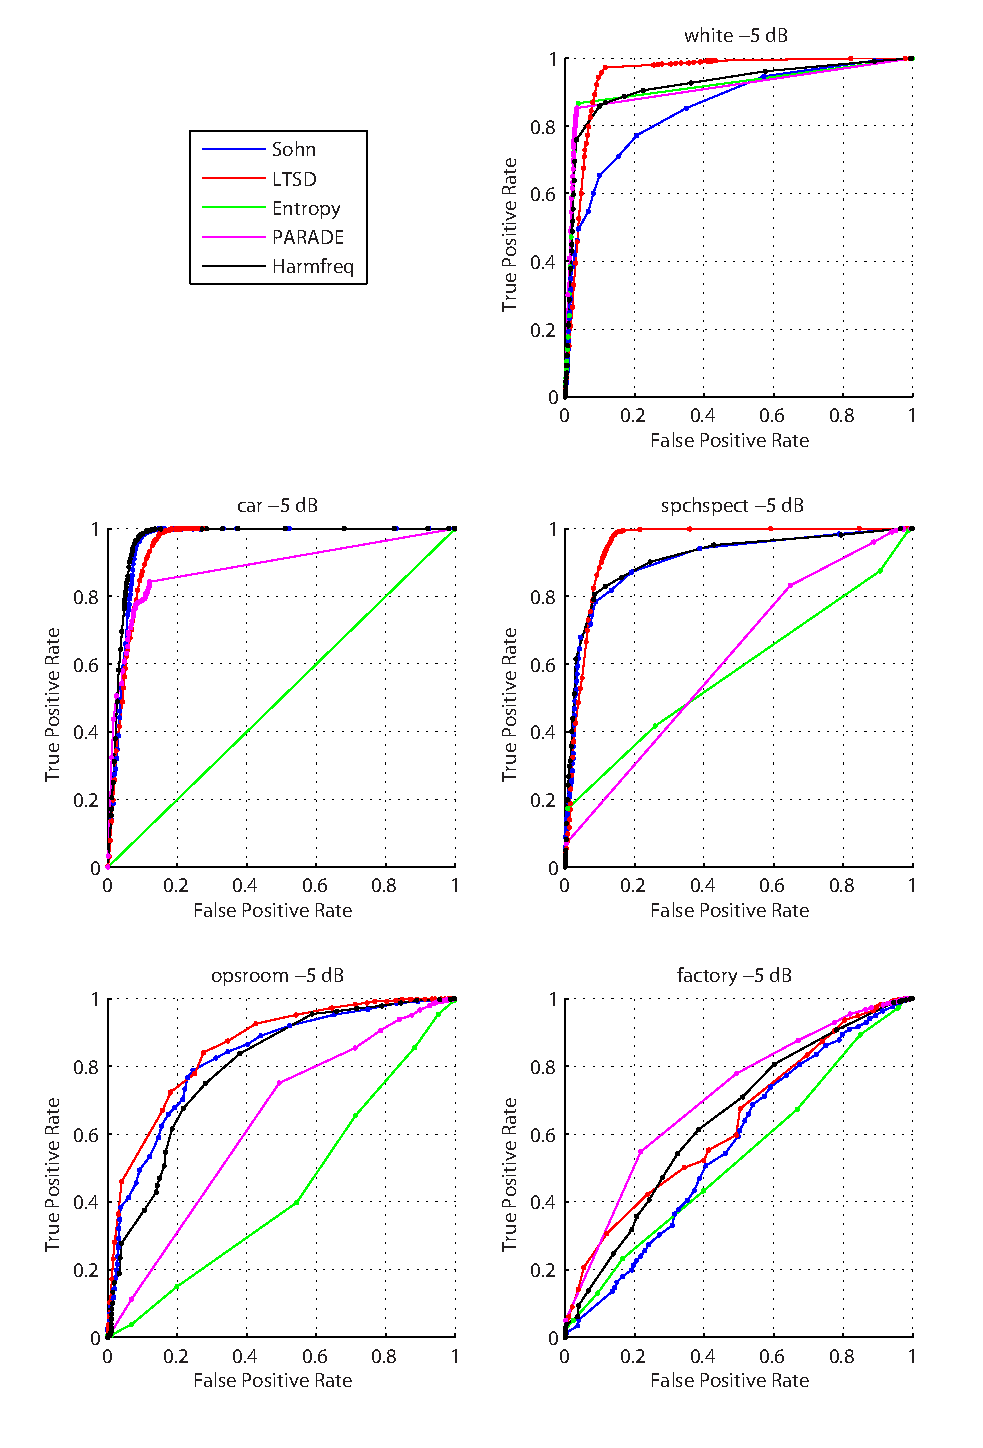
\includegraphics[width=1.0\columnwidth]{Figures/Chapter3/-5dBh.pdf}
		\rule{37em}{0.5pt}
	\caption[ROC curves of the evaluated algorithms \emph{with} hang-over under -5 dB SNR]{ROC curves of the evaluated VAD algorithms \emph{with} hang-over under -5 dB SNR}
	\label{fig:-5dBh}
\end{figure}

\begin{figure}[htbp]
	\centering
		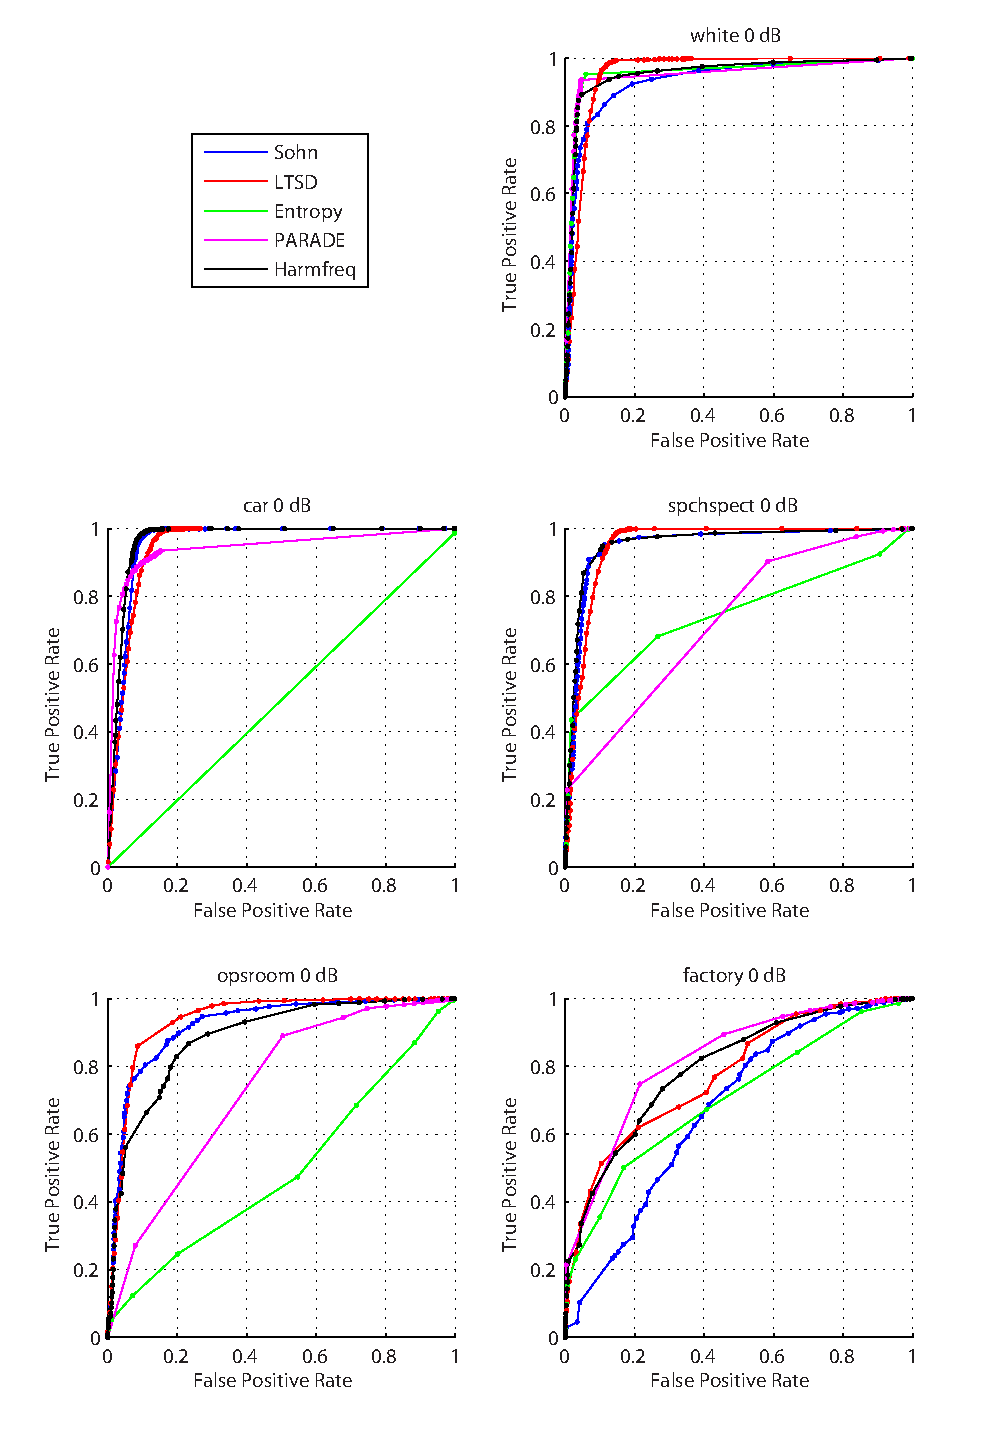
\includegraphics[width=1.0\columnwidth]{Figures/Chapter3/0dBh.pdf}
		\rule{37em}{0.5pt}
	\caption[ROC curves of the evaluated algorithms \emph{with} hang-over under 0 dB SNR]{ROC curves of the evaluated VAD algorithms \emph{with} hang-over under 0 dB SNR}
	\label{fig:0dBh}
\end{figure}

\begin{figure}[htbp]
	\centering
		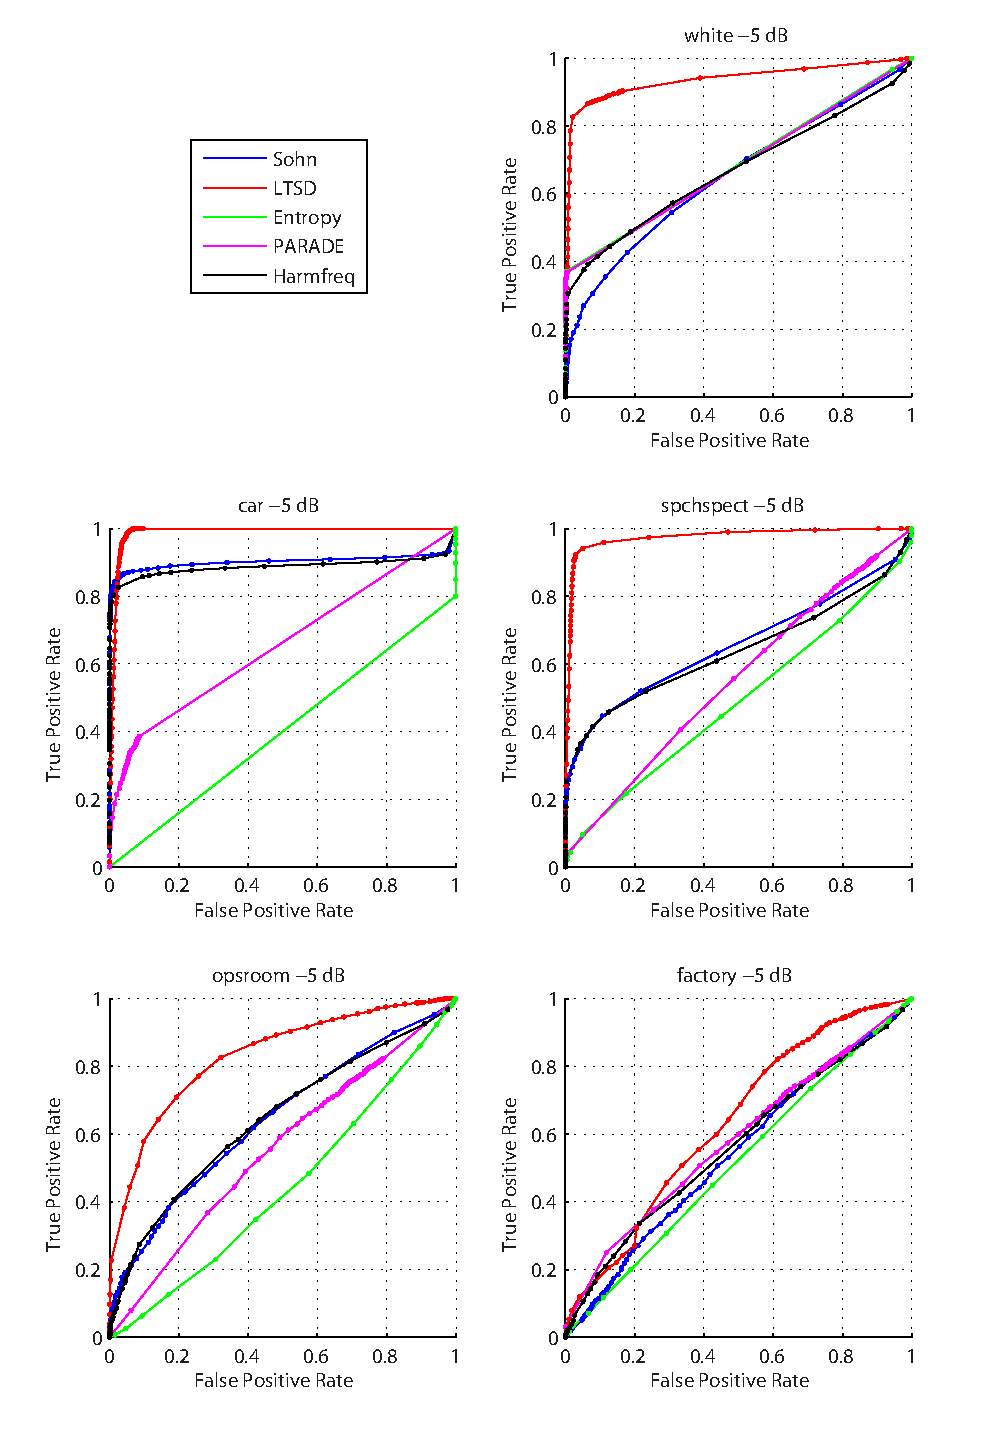
\includegraphics[width=1.0\columnwidth]{Figures/Chapter3/-5dBnoh.pdf}
		\rule{37em}{0.5pt}
	\caption[ROC curves of the evaluated algorithms \emph{without} hang-over under -5 dB SNR]{ROC curves of the evaluated VAD algorithms \emph{without} hang-over under -5 dB SNR}
	\label{fig:-5dBnoh}
\end{figure}

\begin{figure}[htbp]
	\centering
		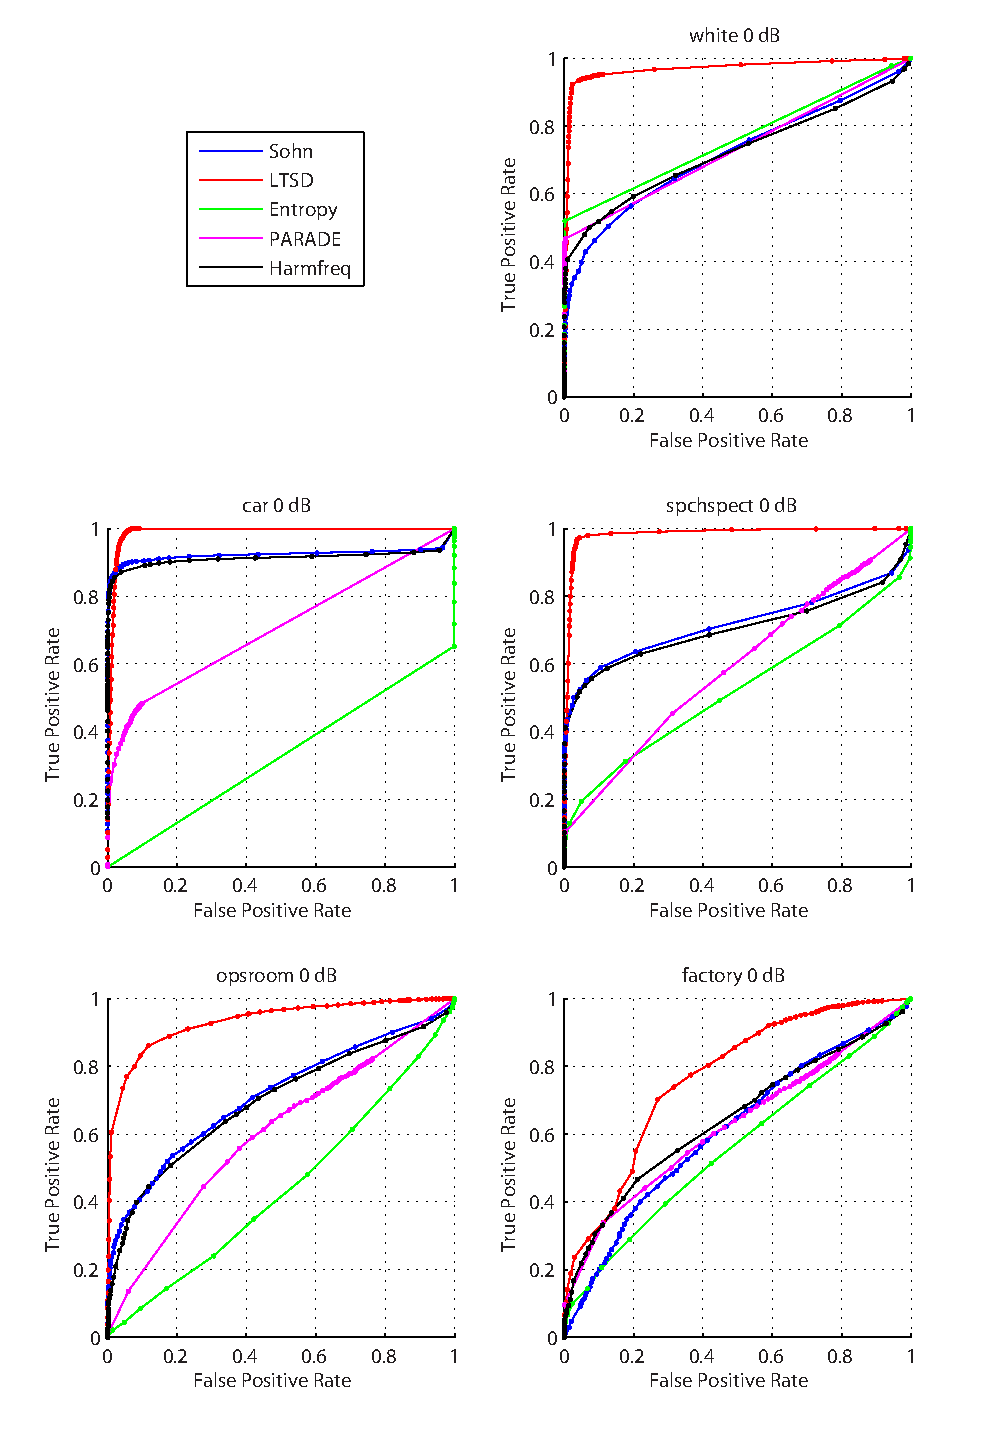
\includegraphics[width=1.0\columnwidth]{Figures/Chapter3/0dBnoh.pdf}
		\rule{37em}{0.5pt}
	\caption[ROC curves of the evaluated algorithms \emph{without} hang-over under 0 dB SNR]{ROC curves of the evaluated VAD algorithms \emph{without} hang-over under 0 dB SNR}
	\label{fig:0dBnoh}
\end{figure}